\documentclass{report}

\usepackage{hyperref}

\usepackage{epstopdf}
\usepackage{amsmath}
\usepackage{amssymb}
\usepackage{subfig}
%\usepackage{multirow}
\usepackage[utf8]{inputenc}
\usepackage[T1]{fontenc}
\usepackage{standalone}
\usepackage{tikz}
\usepackage{tabularx}
\usepackage{float}
\usepackage[section]{placeins}
\usepackage{sverb}
\usepackage{import}
\usepackage{verbatim}
\usepackage{listings}
\usepackage{xcolor}

\graphicspath{{img/}}
\DeclareGraphicsExtensions{.pdf,.png,.jpg,.svg} %For pdflatex






\begin{document}

\begin{titlepage}
    \begin{center}
        
\includegraphics[width=.50\linewidth]{other/polsl.png}\\
        \Huge
        \textbf{Przetwarzanie Obrazów Cyfrowych}
        \\ \vspace{1.5cm}
        \Large
        \textbf{Raport z ćwiczenia nr. 6: } \\
        % \textbf{WSTĘPNE PRZETWARZANIE OBRAZÓW — FILTRY LINIOWE}
        \textbf{Wstępne przetwarzanie obrazów - filtry liniowe}        
    \end{center}
    \vspace{3.0cm}
    \Large
    Raport opracował: \\
    Dawid Kania \\
    Grupa 6 Semestr 6 \\ \\
    Data wykonania ćwiczenia: 09.06.2022
\end{titlepage}
 



\section*{Binaryzacja obrazów}

\newcommand{\ww}{0.24}
\begin{figure}[H]
    \captionsetup[subfloat]{justification=raggedright,singlelinecheck=false, position=bottom,labelformat=empty} %
    \subfloat[256 poziomów szarości                        ]{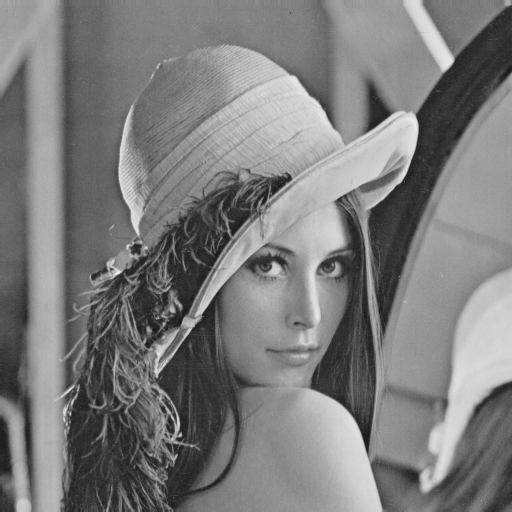
\includegraphics[width=\ww\linewidth]{../img/q2/i1/orig.png}} \hfill%	
    \subfloat[Wynik binaryzacji metodą Otsu                ]{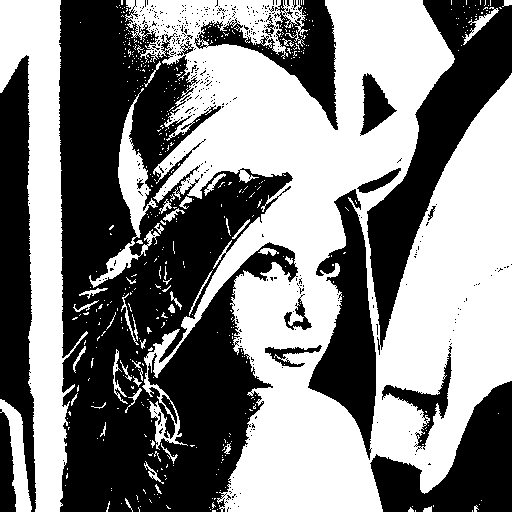
\includegraphics[width=\ww\linewidth]{../img/q2/i1/OTSU.png}} \hfill% wypełnenie
    \subfloat[Wynik Dithreringu metodą FS - własny skrypt  ]{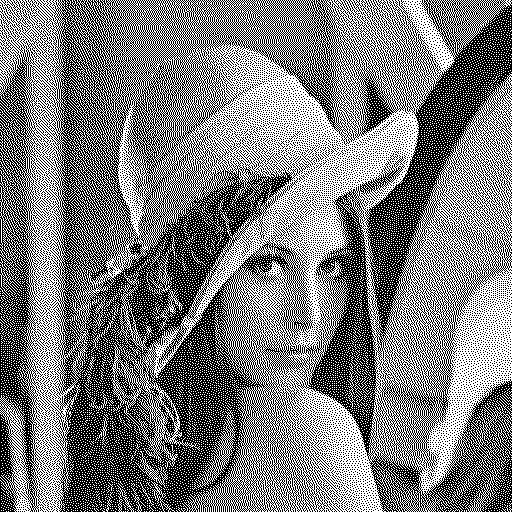
\includegraphics[width=\ww\linewidth]{../img/q2/i1/FS__.png}} \hfill
    \subfloat[Wynik Dithreringu metodą FS - inna aplikacja ]{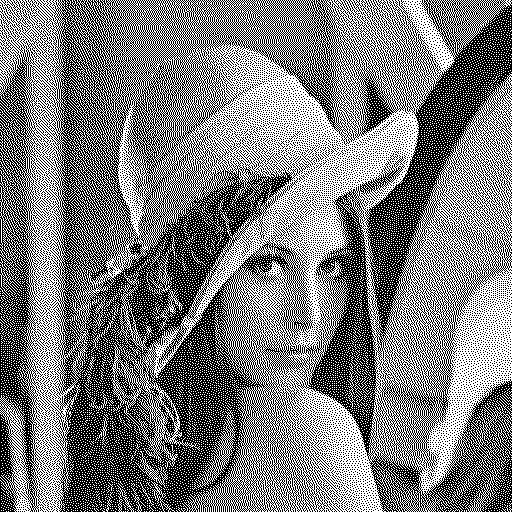
\includegraphics[width=\ww\linewidth]{../img/q2/i1/FS__.png}} \\
    \subfloat[256 poziomów szarości                        ]{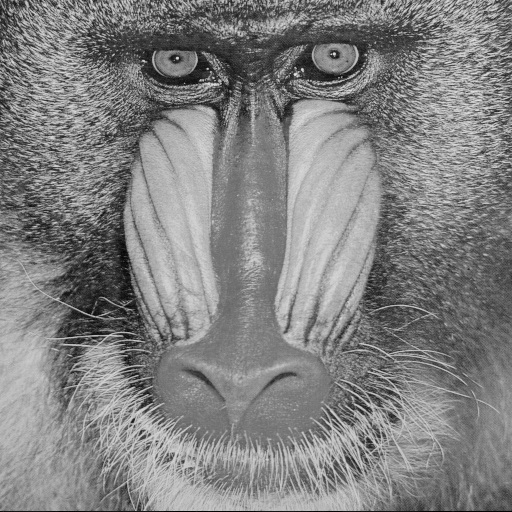
\includegraphics[width=\ww\linewidth]{../img/q2/i2/orig.png}} \hfill%	
    \subfloat[Wynik binaryzacji metodą Otsu                ]{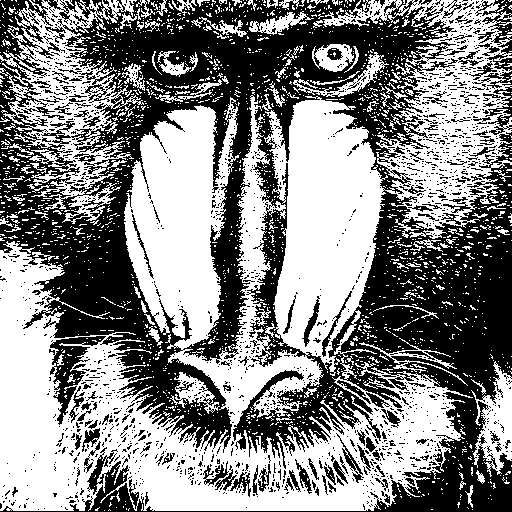
\includegraphics[width=\ww\linewidth]{../img/q2/i2/OTSU.png}} \hfill% wypełnenie
    \subfloat[Wynik Dithreringu metodą FS - własny skrypt  ]{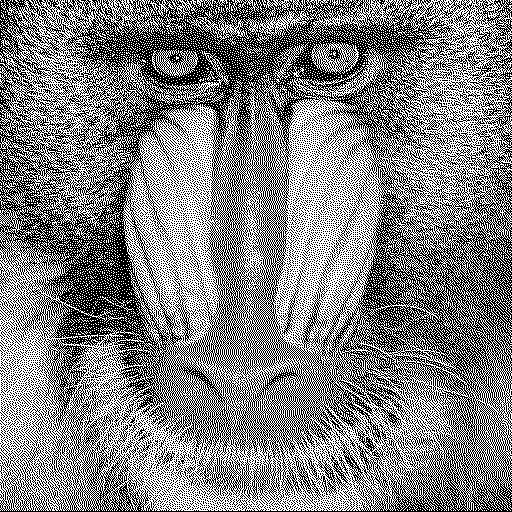
\includegraphics[width=\ww\linewidth]{../img/q2/i2/FS__.png}} \hfill
    \subfloat[Wynik Dithreringu metodą FS - inna aplikacja ]{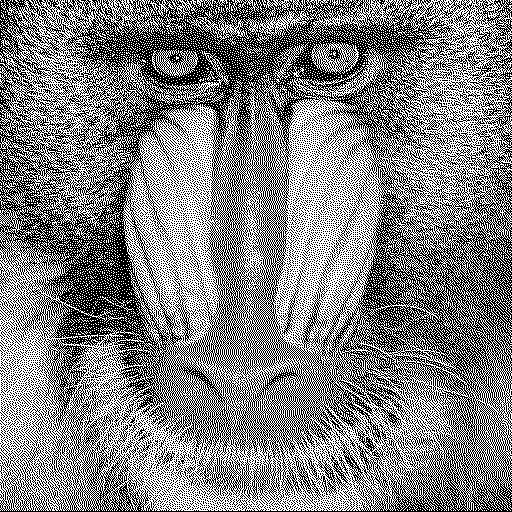
\includegraphics[width=\ww\linewidth]{../img/q2/i2/FS__.png}} 
    \caption{Tekst do zmiany} 
    \label{fig:porownanie1}
\end{figure}

\begin{figure}[H]
    \captionsetup[subfloat]{justification=raggedright,singlelinecheck=false, position=bottom,labelformat=empty} %
    \subfloat[256 poziomów szarości                        ]{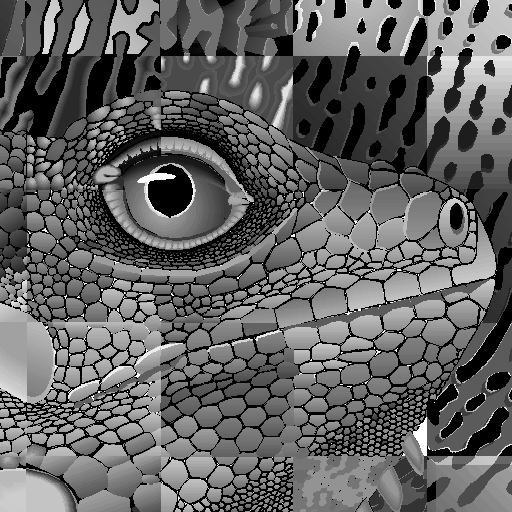
\includegraphics[width=\ww\linewidth]{../img/q2/i3/orig.png}} \hfill%	
    \subfloat[Wynik binaryzacji metodą Otsu                ]{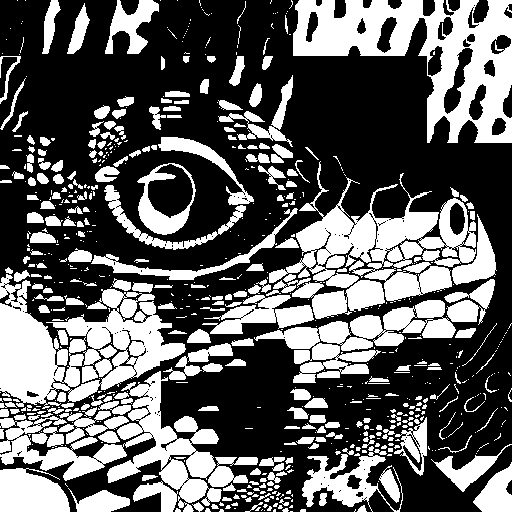
\includegraphics[width=\ww\linewidth]{../img/q2/i3/OTSU.png}} \hfill% wypełnenie
    \subfloat[Wynik Dithreringu metodą FS - własny skrypt  ]{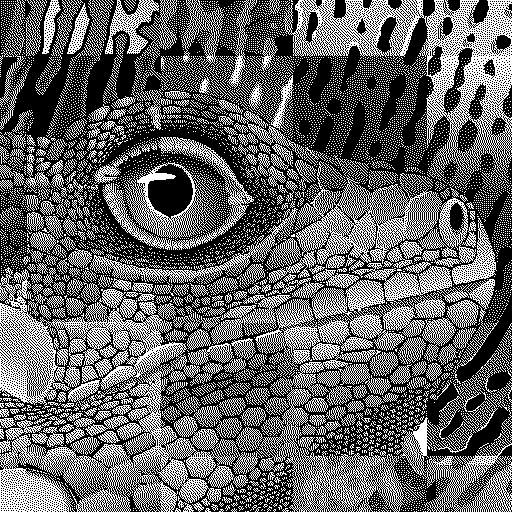
\includegraphics[width=\ww\linewidth]{../img/q2/i3/FS__.png}} \hfill
    \subfloat[Wynik Dithreringu metodą FS - inna aplikacja ]{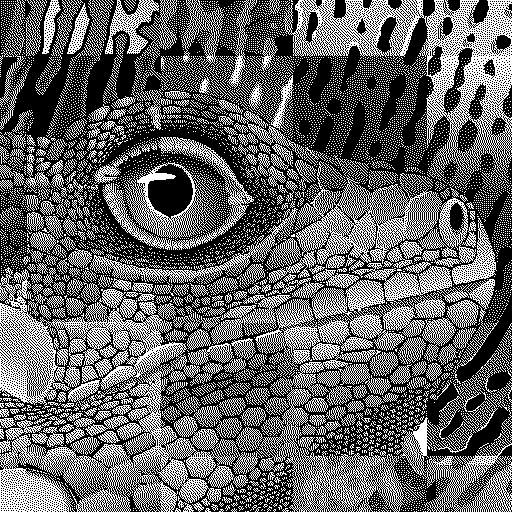
\includegraphics[width=\ww\linewidth]{../img/q2/i3/FS__.png}} \\
    \subfloat[256 poziomów szarości                        ]{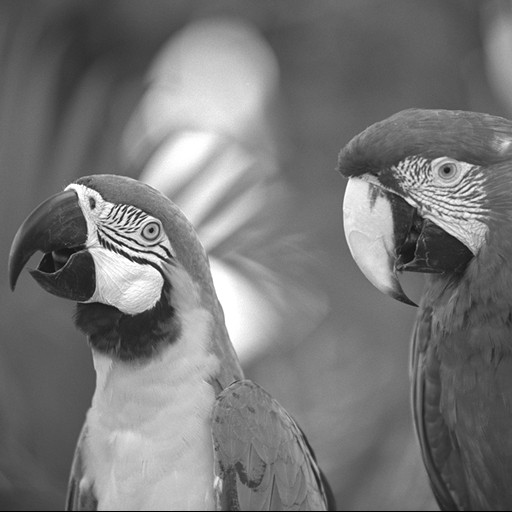
\includegraphics[width=\ww\linewidth]{../img/q2/i4/orig.png}} \hfill%	
    \subfloat[Wynik binaryzacji metodą Otsu                ]{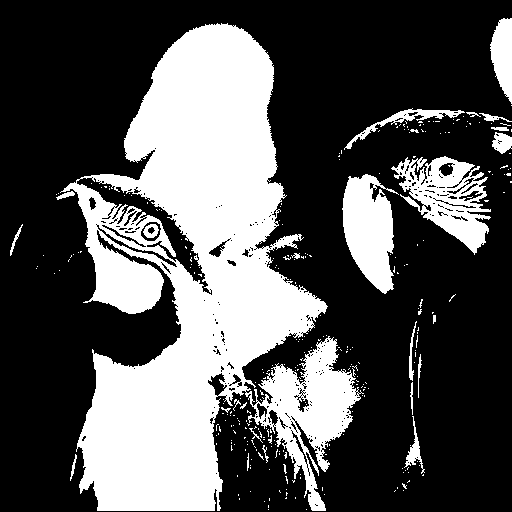
\includegraphics[width=\ww\linewidth]{../img/q2/i4/OTSU.png}} \hfill% wypełnenie
    \subfloat[Wynik Dithreringu metodą FS - własny skrypt  ]{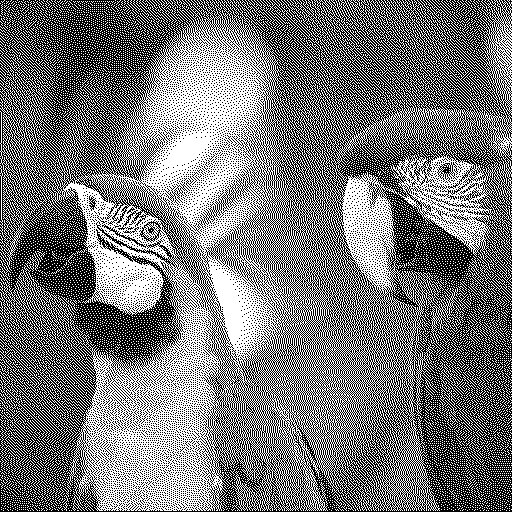
\includegraphics[width=\ww\linewidth]{../img/q2/i4/FS__.png}} \hfill
    \subfloat[Wynik Dithreringu metodą FS - inna aplikacja ]{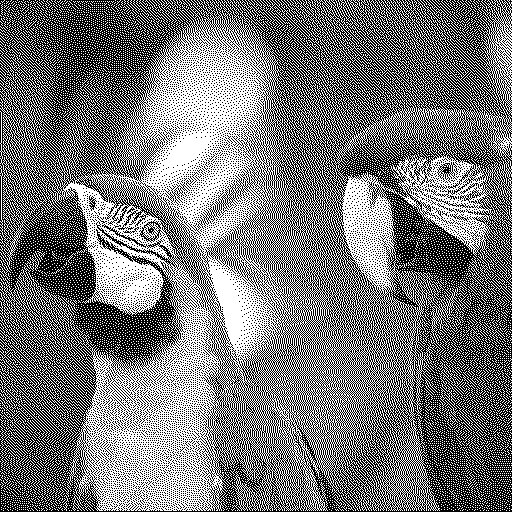
\includegraphics[width=\ww\linewidth]{../img/q2/i4/FS__.png}} 
    \caption{Tekst do zmiany} 
    \label{fig:porownanie2}
\end{figure}

\begin{figure}[H]
    \captionsetup[subfloat]{justification=raggedright,singlelinecheck=false, position=bottom,labelformat=empty} %
    \subfloat[256 poziomów szarości                        ]{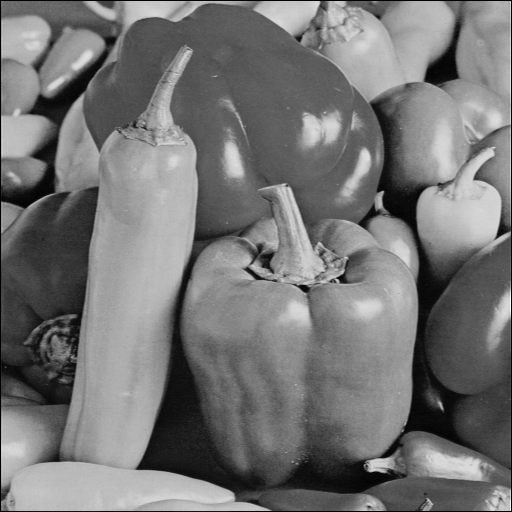
\includegraphics[width=\ww\linewidth]{../img/q2/i5/orig.png}} \hfill%	
    \subfloat[Wynik binaryzacji metodą Otsu                ]{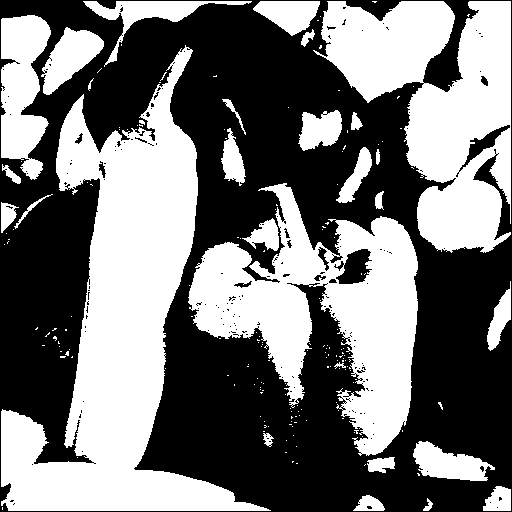
\includegraphics[width=\ww\linewidth]{../img/q2/i5/OTSU.png}} \hfill% wypełnenie
    \subfloat[Wynik Dithreringu metodą FS - własny skrypt  ]{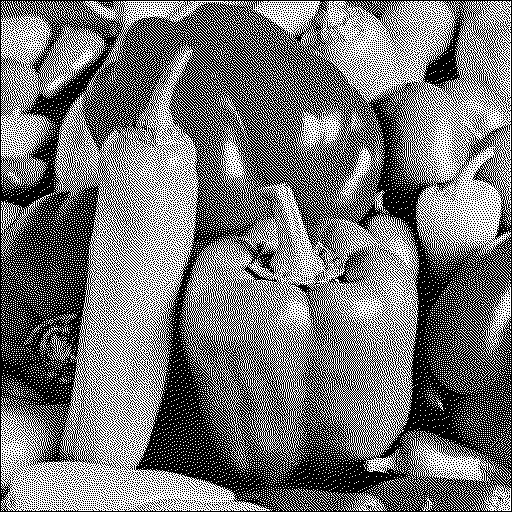
\includegraphics[width=\ww\linewidth]{../img/q2/i5/FS__.png}} \hfill
    \subfloat[Wynik Dithreringu metodą FS - inna aplikacja ]{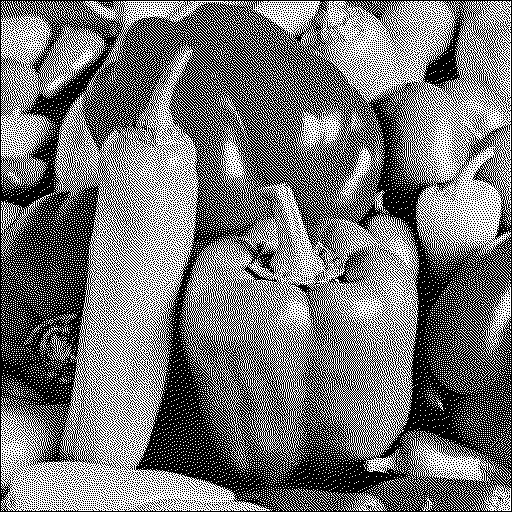
\includegraphics[width=\ww\linewidth]{../img/q2/i5/FS__.png}} \\
    \subfloat[256 poziomów szarości                        ]{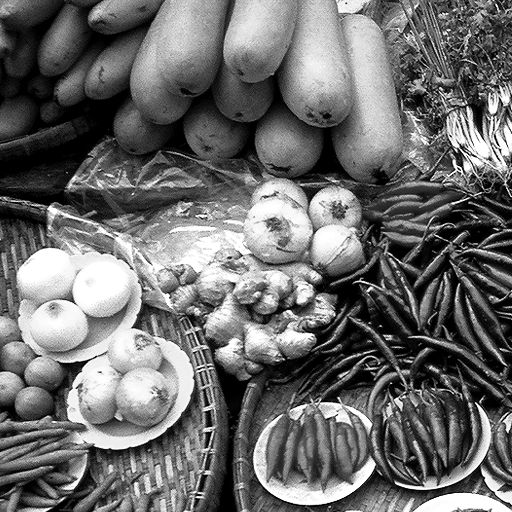
\includegraphics[width=\ww\linewidth]{../img/q2/i6/orig.png}} \hfill%	
    \subfloat[Wynik binaryzacji metodą Otsu                ]{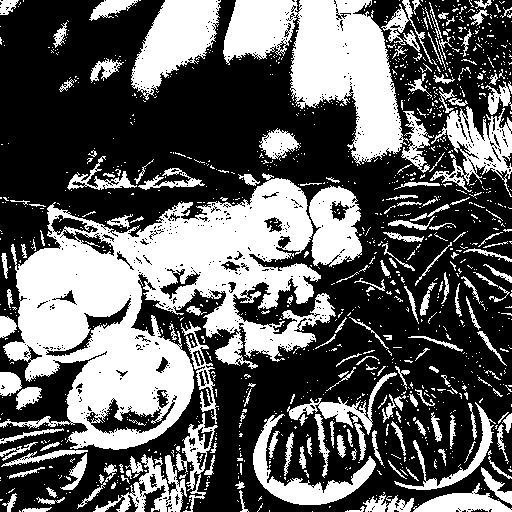
\includegraphics[width=\ww\linewidth]{../img/q2/i6/OTSU.png}} \hfill% wypełnenie
    \subfloat[Wynik Dithreringu metodą FS - własny skrypt  ]{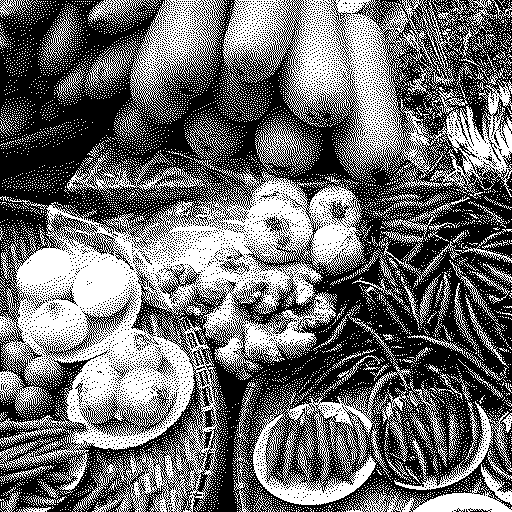
\includegraphics[width=\ww\linewidth]{../img/q2/i6/FS__.png}} \hfill
    \subfloat[Wynik Dithreringu metodą FS - inna aplikacja ]{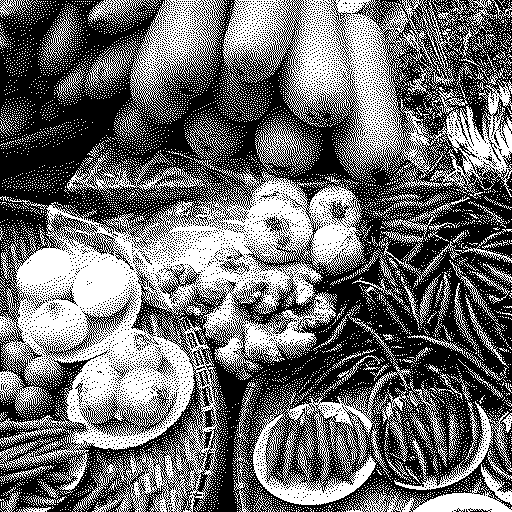
\includegraphics[width=\ww\linewidth]{../img/q2/i6/FS__.png}} 
    \caption{Tekst do zmiany} 
    \label{fig:porownanie3}
\end{figure}


\section*{Kwantyzacja obrazów na 16 kolorów}


\begin{figure}[H]
    \captionsetup[subfloat]{justification=raggedright,singlelinecheck=false, position=bottom,labelformat=empty} %
    \subfloat["True color"                                  ]{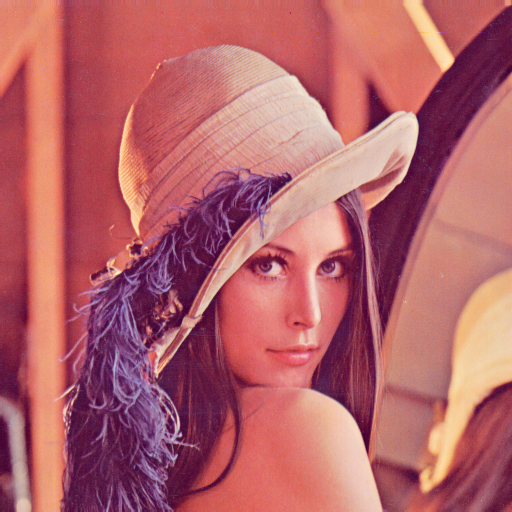
\includegraphics[width=\ww\linewidth]{../img/q16/i1/origi.png}} \hfill%	
    \subfloat[Kwantyzacja na 16 barw bez ditheringu         ]{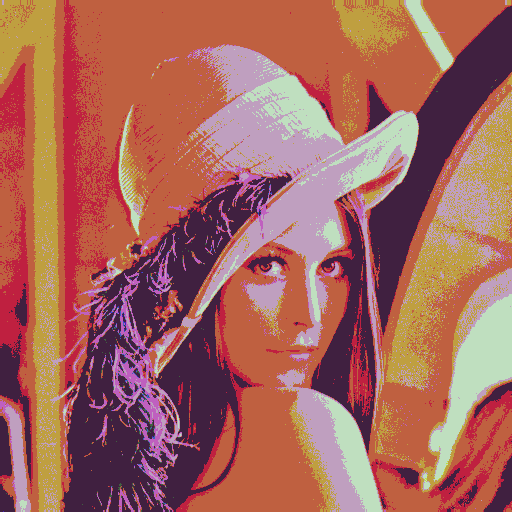
\includegraphics[width=\ww\linewidth]{../img/q16/i1/QU_16.png}} \hfill% wypełnenie
    \subfloat[Wynik Dithreringu metodą FS - własny skrypt   ]{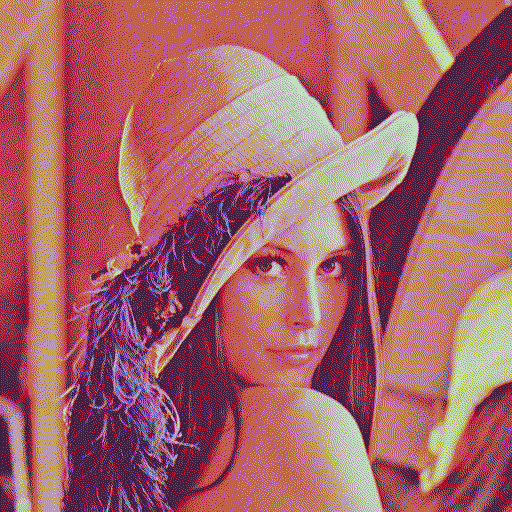
\includegraphics[width=\ww\linewidth]{../img/q16/i1/FS_16.png}} \hfill
    \subfloat[Wynik Dithreringu metodą FS - inna aplikacja  ]{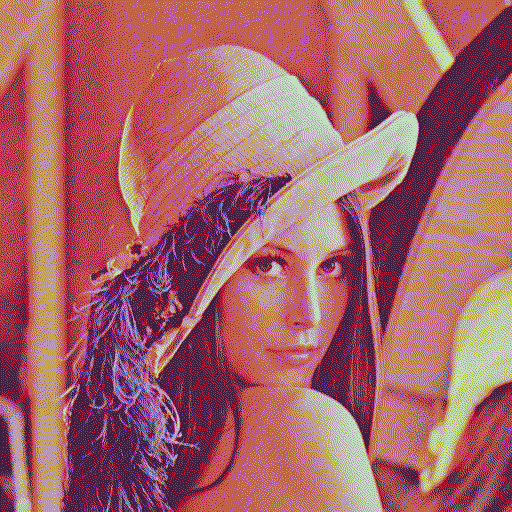
\includegraphics[width=\ww\linewidth]{../img/q16/i1/FS_16.png}} \\
    \subfloat[                                              ]{
\includegraphics[width=\ww\linewidth]{other/Empty.png}} \hfill
    \subfloat[Kwantyzacja na 256 barw bez ditheringu        ]{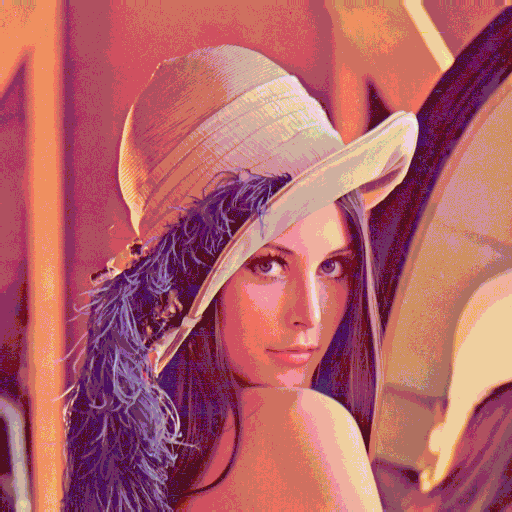
\includegraphics[width=\ww\linewidth]{../img/q16/i1/QU256.png}} \hfill
    \subfloat[Wynik Dithreringu metodą FS - własny skrypt   ]{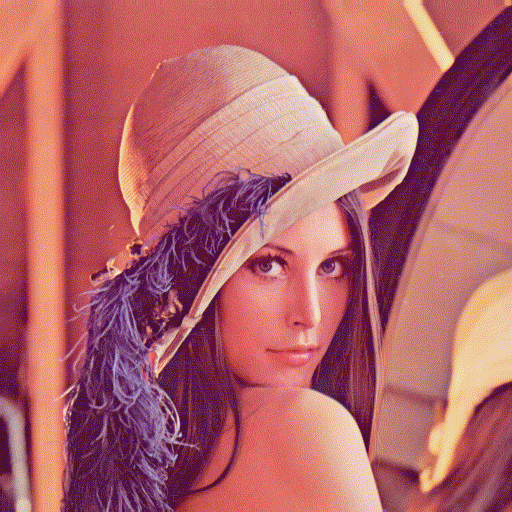
\includegraphics[width=\ww\linewidth]{../img/q16/i1/FS256.png}} \hfill% wypełnenie
    \subfloat[Wynik Dithreringu metodą FS - inna aplikacja  ]{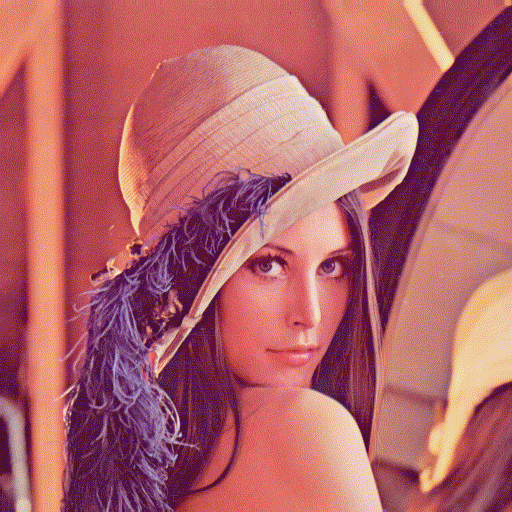
\includegraphics[width=\ww\linewidth]{../img/q16/i1/FS256.png}} 
    \caption{Tekst do zmiany} 
    \label{fig:porownanie4}
\end{figure}

\begin{figure}[H]
    \captionsetup[subfloat]{justification=raggedright,singlelinecheck=false, position=bottom,labelformat=empty} %
    \subfloat["True color"                                  ]{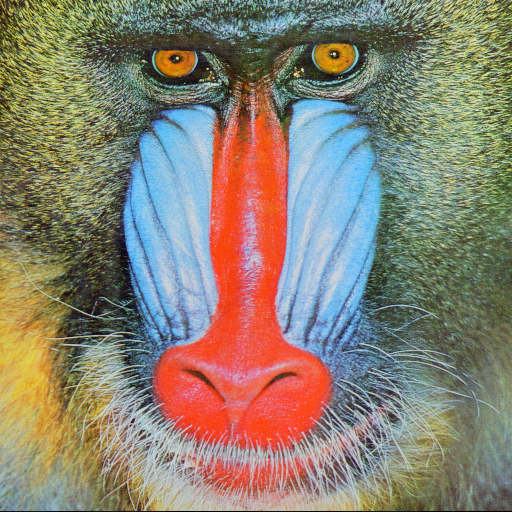
\includegraphics[width=\ww\linewidth]{../img/q16/i2/origi.png}} \hfill%	
    \subfloat[Kwantyzacja na 16 barw bez ditheringu         ]{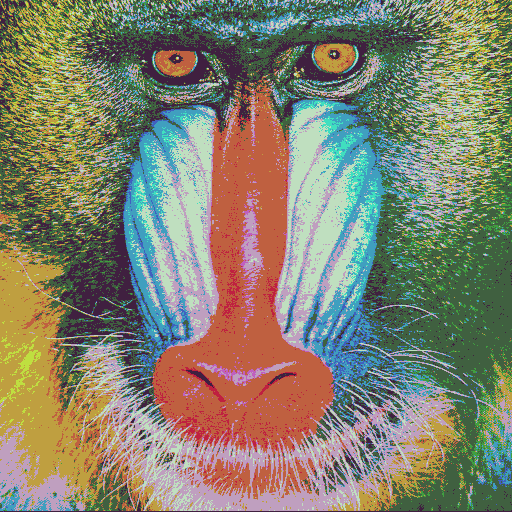
\includegraphics[width=\ww\linewidth]{../img/q16/i2/QU_16.png}} \hfill% wypełnenie
    \subfloat[Wynik Dithreringu metodą FS - własny skrypt   ]{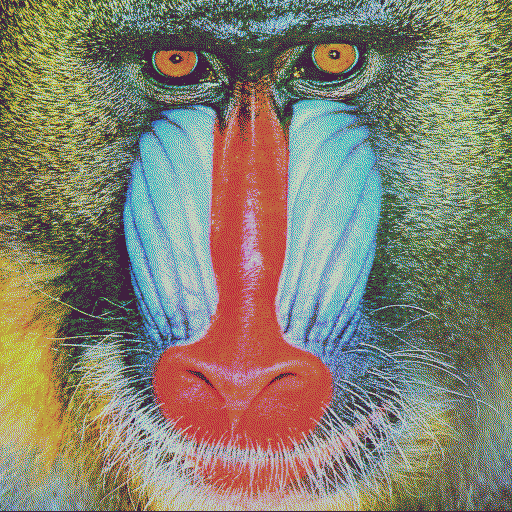
\includegraphics[width=\ww\linewidth]{../img/q16/i2/FS_16.png}} \hfill
    \subfloat[Wynik Dithreringu metodą FS - inna aplikacja  ]{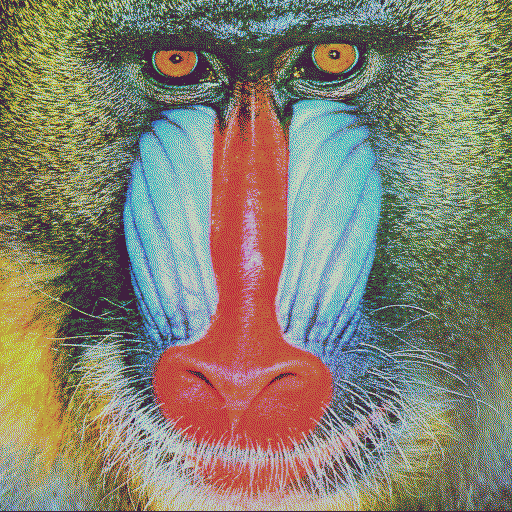
\includegraphics[width=\ww\linewidth]{../img/q16/i2/FS_16.png}} \\
    \subfloat[                                              ]{
\includegraphics[width=\ww\linewidth]{other/Empty.png}} \hfill
    \subfloat[Kwantyzacja na 256 barw bez ditheringu        ]{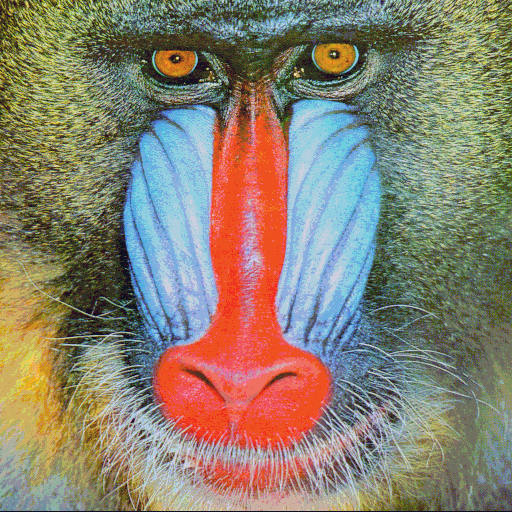
\includegraphics[width=\ww\linewidth]{../img/q16/i2/QU256.png}} \hfill
    \subfloat[Wynik Dithreringu metodą FS - własny skrypt   ]{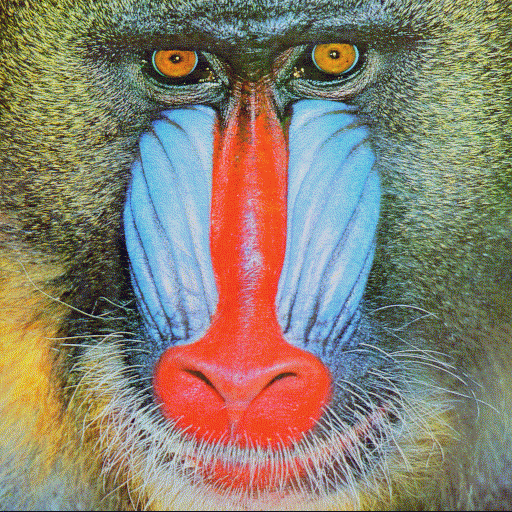
\includegraphics[width=\ww\linewidth]{../img/q16/i2/FS256.png}} \hfill% wypełnenie
    \subfloat[Wynik Dithreringu metodą FS - inna aplikacja  ]{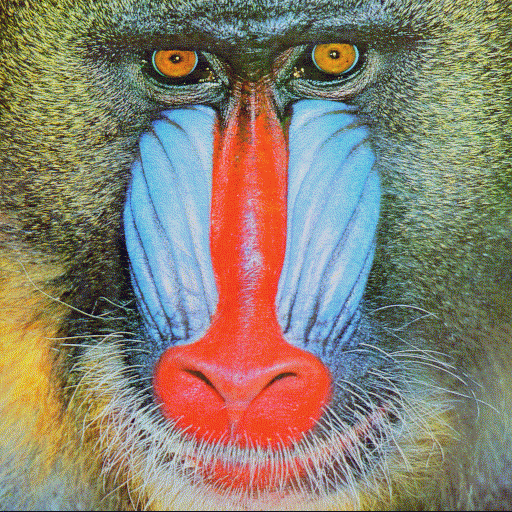
\includegraphics[width=\ww\linewidth]{../img/q16/i2/FS256.png}} 
    \caption{Tekst do zmiany} 
    \label{fig:porownanie5}
\end{figure}


\begin{figure}[H]
    \captionsetup[subfloat]{justification=raggedright,singlelinecheck=false, position=bottom,labelformat=empty} %
    \subfloat["True color"                                  ]{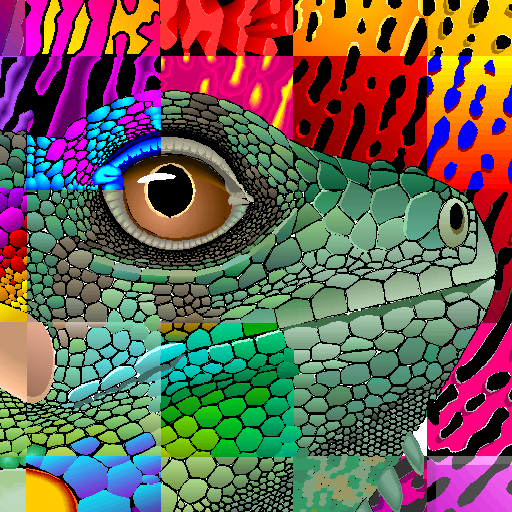
\includegraphics[width=\ww\linewidth]{../img/q16/i3/origi.png}} \hfill%	
    \subfloat[Kwantyzacja na 16 barw bez ditheringu         ]{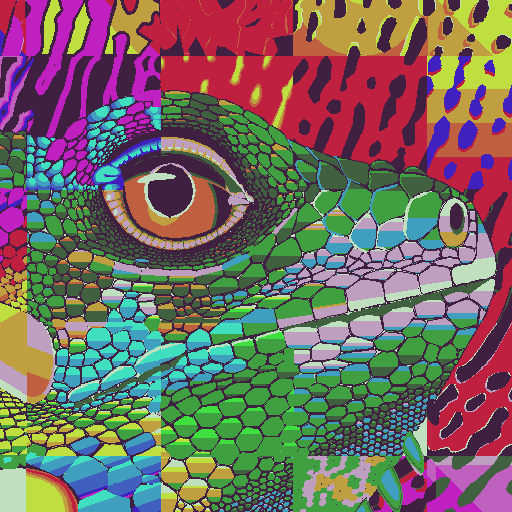
\includegraphics[width=\ww\linewidth]{../img/q16/i3/QU_16.png}} \hfill% wypełnenie
    \subfloat[Wynik Dithreringu metodą FS - własny skrypt   ]{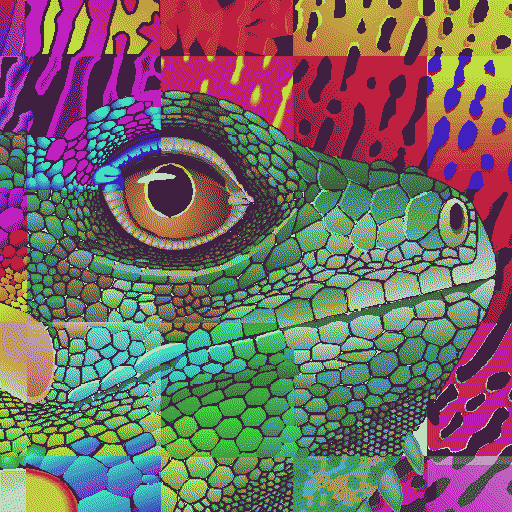
\includegraphics[width=\ww\linewidth]{../img/q16/i3/FS_16.png}} \hfill
    \subfloat[Wynik Dithreringu metodą FS - inna aplikacja  ]{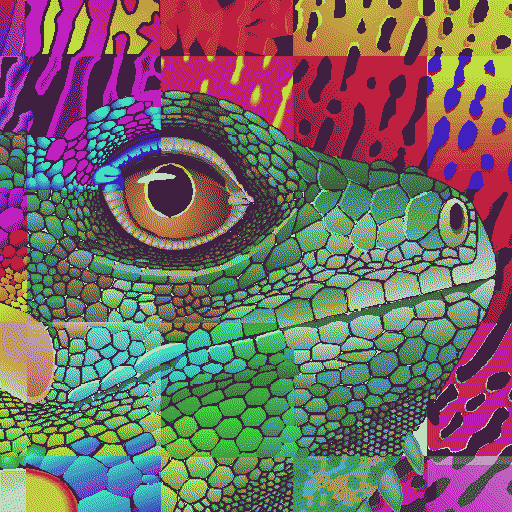
\includegraphics[width=\ww\linewidth]{../img/q16/i3/FS_16.png}} \\
    \subfloat[                                              ]{
\includegraphics[width=\ww\linewidth]{other/Empty.png}} \hfill
    \subfloat[Kwantyzacja na 256 barw bez ditheringu        ]{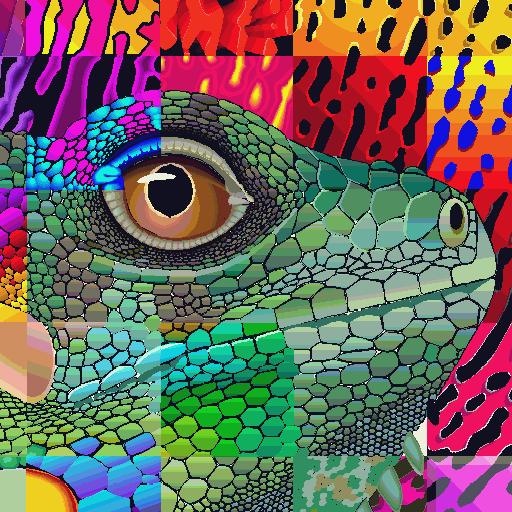
\includegraphics[width=\ww\linewidth]{../img/q16/i3/QU256.png}} \hfill
    \subfloat[Wynik Dithreringu metodą FS - własny skrypt   ]{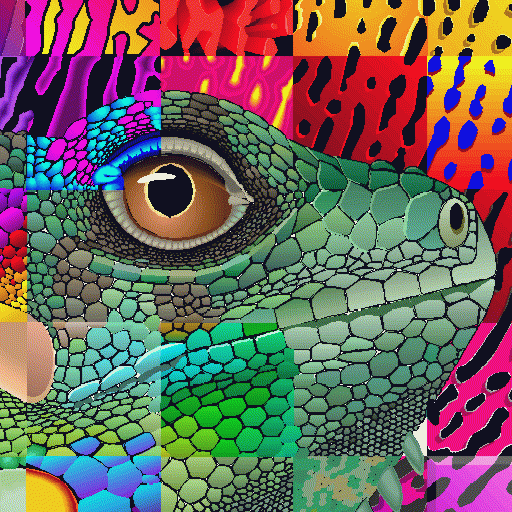
\includegraphics[width=\ww\linewidth]{../img/q16/i3/FS256.png}} \hfill% wypełnenie
    \subfloat[Wynik Dithreringu metodą FS - inna aplikacja  ]{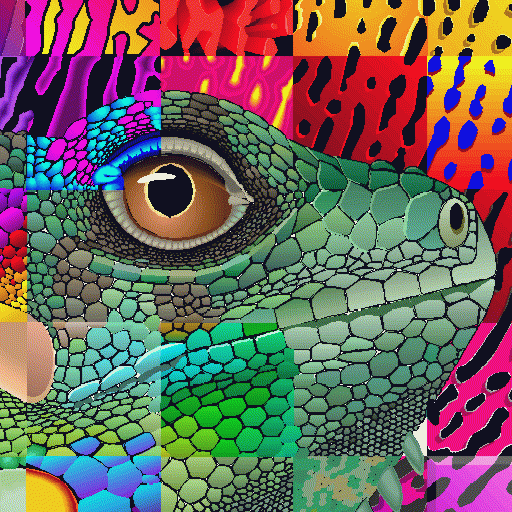
\includegraphics[width=\ww\linewidth]{../img/q16/i3/FS256.png}} 
    \caption{Tekst do zmiany} 
    \label{fig:porownanie6}
\end{figure}


\begin{figure}[H]
    \captionsetup[subfloat]{justification=raggedright,singlelinecheck=false, position=bottom,labelformat=empty} %
    \subfloat["True color"                                  ]{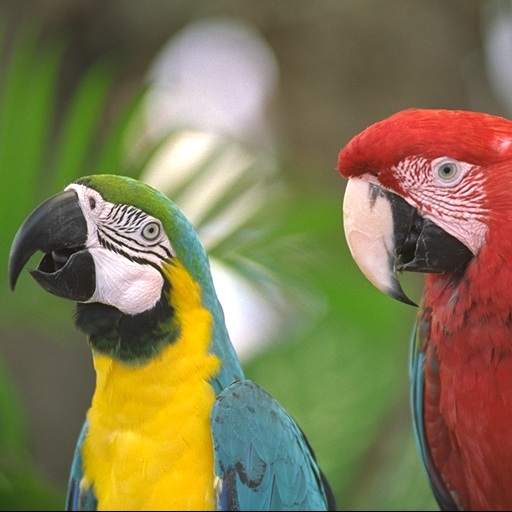
\includegraphics[width=\ww\linewidth]{../img/q16/i4/origi.png}} \hfill%	
    \subfloat[Kwantyzacja na 16 barw bez ditheringu         ]{\includegraphics[width=\ww\linewidth]{../img/q16/i4/QU_16.png}} \hfill% wypełnenie
    \subfloat[Wynik Dithreringu metodą FS - własny skrypt   ]{\includegraphics[width=\ww\linewidth]{../img/q16/i4/FS_16.png}} \hfill
    \subfloat[Wynik Dithreringu metodą FS - inna aplikacja  ]{\includegraphics[width=\ww\linewidth]{../img/q16/i4/FS_16.png}} \\
    \subfloat[                                              ]{\includegraphics[width=\ww\linewidth]{other/Empty.png}} \hfill
    \subfloat[Kwantyzacja na 256 barw bez ditheringu        ]{\includegraphics[width=\ww\linewidth]{../img/q16/i4/QU256.png}} \hfill
    \subfloat[Wynik Dithreringu metodą FS - własny skrypt   ]{\includegraphics[width=\ww\linewidth]{../img/q16/i4/FS256.png}} \hfill% wypełnenie
    \subfloat[Wynik Dithreringu metodą FS - inna aplikacja  ]{\includegraphics[width=\ww\linewidth]{../img/q16/i4/FS256.png}} 
    \caption{Tekst do zmiany} 
    \label{fig:porownanie7}
\end{figure}


\begin{figure}[H]
    \captionsetup[subfloat]{justification=raggedright,singlelinecheck=false, position=bottom,labelformat=empty} %
    \subfloat["True color"                                  ]{\includegraphics[width=\ww\linewidth]{../img/q16/i5/origi.png}} \hfill%	
    \subfloat[Kwantyzacja na 16 barw bez ditheringu         ]{\includegraphics[width=\ww\linewidth]{../img/q16/i5/QU_16.png}} \hfill% wypełnenie
    \subfloat[Wynik Dithreringu metodą FS - własny skrypt   ]{\includegraphics[width=\ww\linewidth]{../img/q16/i5/FS_16.png}} \hfill
    \subfloat[Wynik Dithreringu metodą FS - inna aplikacja  ]{\includegraphics[width=\ww\linewidth]{../img/q16/i5/FS_16.png}} \\
    \subfloat[                                              ]{\includegraphics[width=\ww\linewidth]{other/Empty.png}} \hfill
    \subfloat[Kwantyzacja na 256 barw bez ditheringu        ]{\includegraphics[width=\ww\linewidth]{../img/q16/i5/QU256.png}} \hfill
    \subfloat[Wynik Dithreringu metodą FS - własny skrypt   ]{\includegraphics[width=\ww\linewidth]{../img/q16/i5/FS256.png}} \hfill% wypełnenie
    \subfloat[Wynik Dithreringu metodą FS - inna aplikacja  ]{\includegraphics[width=\ww\linewidth]{../img/q16/i5/FS256.png}} 
    \caption{Tekst do zmiany} 
    \label{fig:porownanie8}
\end{figure}


\section*{Podsumowanie wyników}


\begin{table}[H]
    \caption{porównanie wskaźników PSNR po binaryzacji obrazu w skali szarości}
    \centering
    \begin{tabular}{llll}
    \hline
             &           & OTSU   & FS       \\ \hline
    Fig. 1 & lena      & 8.8492 & 6.7044   \\ 
             & baboon    & 8.5275 & 6.6666   \\ 
    Fig. 2 & frymire   & 9.6568 & 7.6910   \\ 
             & kodim23   & 8.9605 & 6.7288   \\ 
    Fig. 3 & peppers3  & 9.4280 & 6.9201   \\ 
             & bangko    & 11.085 & 8.3271   \\ \hline
    \end{tabular}
\end{table}


\begin{table}[H]
    \caption{porównanie wskaźników PSNR po kwantyzacji obrazu}
    \centering
    \begin{tabular}{llllll}
    \hline
           &           & Bez dither.    & FS            & Bez dither.    & FS              \\
           &           & 16 kolorów     & 16 kolorów    & 256 kolorów    & 256 kolorów     \\ \hline
    Fig. 1 & lena      & 18.692         & 16.360        & 25.458         & 23.394          \\ 
    Fig. 2 & baboon    & 18.403         & 16.802        & 26.025         & 24.582          \\ 
    Fig. 3 & frymire   & 15.266         & 14.426        & 23.310         & 22.315          \\ 
    Fig. 4 & kodim23   & 18.908         & 16.582        & 25.293         & 23.122          \\ 
    Fig. 5 & peppers3  & 18.402         & 16.314        & 25.895         & 23.788          \\ \hline
    \end{tabular}
\end{table}




\end{document}